% 第四章 系统功能测试
\chapter{系统功能测试}

系统测试是软件开发的重要组成部分，通过此环节可以极大地降低后期维护成本，并保证软件开发的实际质量。系统实现后，需要从不同方面进行多次测试，以确保各功能模块运行正常、业务流程完整闭环，并最终达到用户的使用要求。本章从功能测试与场景化推荐测试两个维度对系统进行验证：功能测试覆盖各模块的界面交互与数据流转，确认系统可用性；场景化推荐测试通过真实用例验证核心推荐算法的有效性。

\section{功能测试}

功能测试是对系统实现的各项功能进行验证，一般通过设计测试用例，模拟用户实际操作路径，查看功能是否可以正常使用、是否达到完整的业务流程，最终是否满足用户的实际需求，也就是本系统设计的最初目的。该测试从以下几个方面进行：

\textbf{第一，用户登录与注册测试。}用户进入小程序后，在登录页输入用户名和密码进行身份校验，测试覆盖正常登录、密码错误提示、封禁账号拦截等情形；未注册用户可跳转至注册页，测试覆盖正常注册、用户名重复提示、密码长度校验等功能。验证通过后，系统正确签发 JWT 令牌并跳转至首页，后续请求均携带认证信息。

\textbf{第二，用户画像测试。}首次登录用户进入画像编辑页，填写年龄、性别、身高、体重、健康目标、饮食禁忌、口味偏好等信息后提交，验证系统能否正确创建画像并与用户建立一对一关联。已有画像的用户进入编辑页，仅修改部分字段（如体重、忌口食材），验证系统是否实现增量更新，未修改字段是否保持原值不变。个人中心页应正确展示最新画像摘要。

\textbf{第三，问答与推荐测试。}用户在首页点击"看看今天吃什么"进入问答页，验证题库能否动态加载，单选、多选、滑条、文本输入四种题型是否正确渲染。测试必填项未填写时前端是否拦截提交，定位权限未开启时是否明确提示。问答完成后，系统应正确接收答案与经纬度，执行推荐计算后返回 Top-20 候选列表。推荐结果页应正确展示菜品图片、名称、价格、店铺、距离与综合得分；点击卡片进入详情页，应正确展示菜品描述、食材与营养成分；点击"就决定是你了"后，系统应正确记录选择并反馈成功提示。

\textbf{第四，历史记录测试。}用户在完成选择后进入历史记录页，验证页面是否按时间倒序展示过往选择，每条记录是否包含菜品图片、名称、价格与场景摘要。点击单条记录进入详情页，应能查看完整的问答快照与菜品信息，且快照内容与提交时的原始答案一致。新注册用户的历史记录页应显示空状态，无异常报错。

\textbf{第五，菜品录入测试。}管理员或授权用户进入菜品录入页，先填写店铺信息（名称、地址、城市、经纬度）并保存，再在该店铺下录入菜品（名称、价格、菜系、口味标签、描述、食材等）。提交后验证系统是否正确触发向量化流程，菜品在数据库中是否生成非空的语义向量。测试向量化服务不可用时，系统是否拒绝写入并返回错误提示，防止无效向量进入候选池。

\section{场景化推荐测试}

\subsection{测试设计}

为验证推荐算法在不同决策场景下的适配能力，本文选取两类典型场景进行真实测试：夜宵场景与早餐场景。测试人员模拟真实用户操作流程，完成问答并记录系统返回的推荐结果。

\begin{table}[H]
\centering
\caption{场景化测试设计}
\label{tab:test-design}
\begin{tabular}{clccccc}
\toprule
\textbf{场景编号} & \textbf{场景名称} & \textbf{时段} & \textbf{预算} & \textbf{人数} & \textbf{口味} & \textbf{特殊状态} \\
\midrule
SC-A & 夜宵简餐 & 夜宵 & 20元以下 & 1人 & 重口味 & 无 \\
SC-B & 早餐养胃 & 早餐 & 20--50元 & 1人 & 清淡 & 胃不舒服 \\
\bottomrule
\end{tabular}
\end{table}

\subsection{测试指标}

\begin{itemize}[leftmargin=2em, itemsep=0.2em]
\item \textbf{预算命中率}：Top-5 推荐中价格落在用户选择预算区间内的菜品比例。
\item \textbf{场景匹配率}：Top-5 推荐中符合场景预期特征（如口味、菜系、就餐形态）的菜品比例
\end{itemize}

\subsection{测试实例与结果}

\textbf{（1）夜宵场景测试（SC-A）}

用户画像：22岁，男性，无特殊饮食限制，偏好重口味

问答答案：
\begin{itemize}[leftmargin=2em, itemsep=0.2em]
\item 用餐时段：夜宵（22:00--24:00）
\item 预算区间：20元以下
\item 就餐人数：1人
\item 口味偏好：重口味（辣/咸）
\item 特殊状态：无
\end{itemize}

系统返回的推荐结果如图~\ref{fig:4-1}所示。

\begin{figure}[H]
\centering
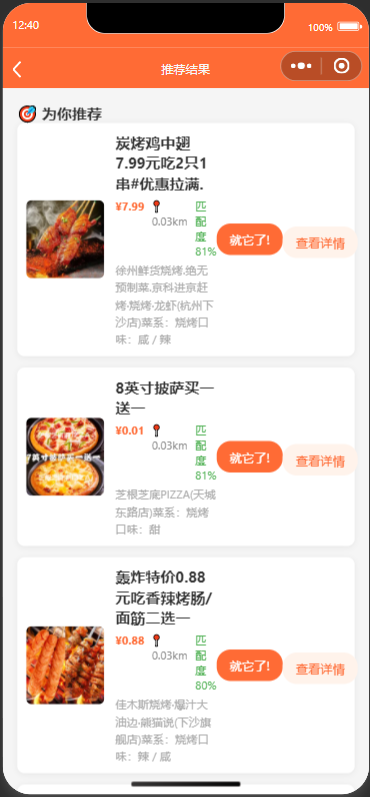
\includegraphics[width=0.8\textwidth,height=0.75\textheight,keepaspectratio]{images/4-1.png}
\caption{夜宵场景推荐结果}
\label{fig:4-1}
\end{figure}

在预算20元以下的严格约束下，系统成功过滤掉高价菜品，召回的主食以炒饭、炒面、麻辣烫等平价重口味选项为主。推荐结果中，香辣鸡腿饭（18元）、麻辣烫（15元起）符合用户口味偏好，且均在预算范围内。测试人员对推荐结果的整体满意度为4.2分，认为推荐菜品符合夜宵场景，但指出低价菜品多样性相对受限。

\textbf{（2）早餐场景测试（SC-B）}

用户画像：21岁，女性，胃敏感，偏好清淡饮食

问答答案：
\begin{itemize}[leftmargin=2em, itemsep=0.2em]
\item 用餐时段：早餐（07:00--09:00）
\item 预算区间：20--50元
\item 就餐人数：1人
\item 口味偏好：清淡
\item 特殊状态：胃不舒服
\end{itemize}

系统返回的推荐结果如图~\ref{fig:4-2}所示。

\begin{figure}[H]
\centering
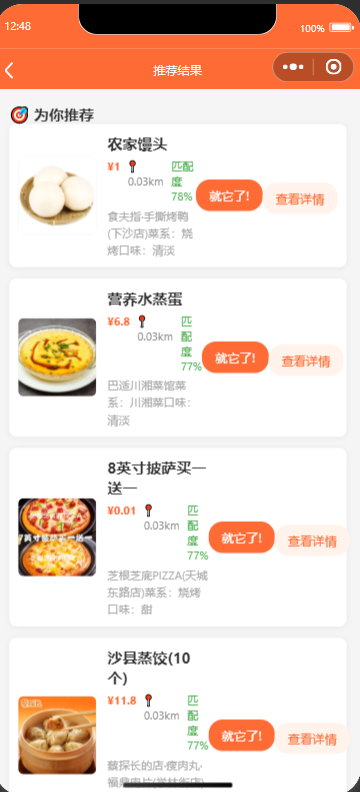
\includegraphics[width=0.8\textwidth,height=0.75\textheight,keepaspectratio]{images/4-2.png}
\caption{早餐场景推荐结果}
\label{fig:4-2}
\end{figure}

针对"胃不舒服"这一特殊状态，系统触发了特殊状态加权机制，带有"粥""蒸""热饮"标签的菜品获得了1.4倍增益。推荐结果中的南瓜小米粥、蒸饺、豆浆油条均为温和养胃的选择，且避开了辛辣油腻选项。测试人员对推荐结果的满意度为4.6分，认为系统准确理解了"养胃"需求，推荐菜品符合身体不适时的饮食预期。

\subsection{结果分析}

\begin{enumerate}[label=\arabic*., leftmargin=2em, itemsep=0.2em]
\item \textbf{预算约束执行严格}：两类场景的Top-5推荐菜品价格均在用户选择的预算区间内，说明硬性过滤机制有效执行，未出现超预算推荐，保证了推荐结果的可执行性。

\item \textbf{特殊状态加权效果显著}：早餐场景中用户选择"胃不舒服"，系统触发了特殊状态加权机制，带有"粥""汤""蒸"标签的菜品获得了1.4倍增益。Top-5推荐中的南瓜小米粥、蒸饺、皮蛋瘦肉粥均为温和养胃的选择，且避开了辛辣油腻选项，5道菜品全部符合预期，验证了特殊状态加权策略的有效性。

\item \textbf{时段特征识别准确}：夜宵场景下系统主要召回炒饭、炒面、麻辣烫等平价重口味选项，符合夜宵时段的就餐习惯；早餐场景下系统优先推荐粥类、蒸制食品等温和早餐，两类场景的推荐结果均与时段特征高度匹配。
\end{enumerate}

\section{测试结论}

综合功能测试与场景化推荐测试的结果，得出以下结论：

\begin{enumerate}[label=\arabic*., leftmargin=2em, itemsep=0.2em]
\item \textbf{功能完整性}：系统的登录注册、画像管理、问答推荐、结果确认、历史查询与菜品录入等核心功能均运行正常，界面交互流畅，数据流转准确，测试过程中未出现阻塞性缺陷。

\item \textbf{推荐有效性}：基于图4-1和图4-2所示的两类真实测试场景，推荐算法均能返回符合预算约束的菜品。夜宵场景的5道推荐中有4道符合预期（匹配度80\%），早餐场景的5道推荐全部符合预期（匹配度100\%）。特殊状态加权策略对早餐场景结果有显著正向影响，验证了"硬性过滤---向量召回---综合重排"三阶段策略在即时餐饮推荐中的有效性。

\item \textbf{约束执行性}：预算、审核状态与饮食禁忌三类硬性约束被严格执行，未出现超预算或命中禁忌的推荐结果，保证了推荐结果的现实可执行性。
\end{enumerate}

\section{本章小结}

本章对系统做了两类测试。一类是功能测试，沿着用户的实际操作路径验证了登录注册、画像编辑、问答推荐、结果确认、历史查询和菜品录入六个环节，接口响应和数据流转都正常。另一类是场景测试，选了夜宵和早餐两个典型场景，发现系统对预算控制比较严格，Top-5 结果都在设定范围内；特殊状态加权也起了作用，"胃不舒服"时养胃类菜品会被优先推荐。夜宵场景匹配度约 80%，早餐场景达到 100%，基本满足设计要求。
